
\section{Designing SimpleSpeech}

\begin{figure}
	\centering
	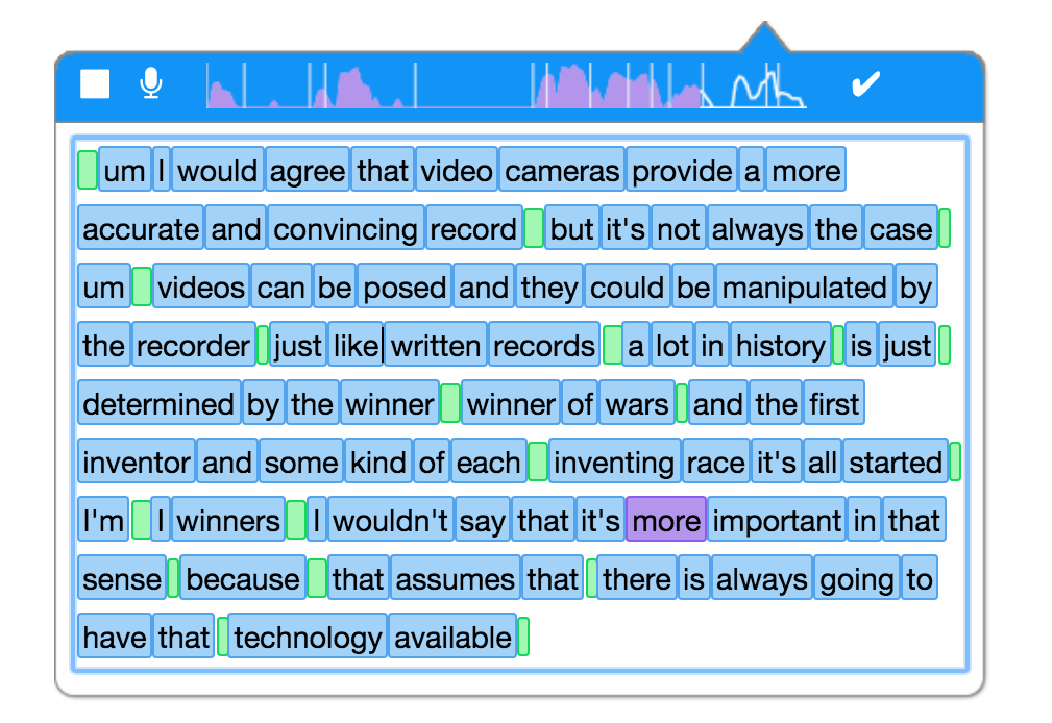
\includegraphics[width=\columnwidth,keepaspectratio]{figures/playback}
	\caption{The waveform visual at the top of the SimpleSpeech editor does not support direct millisecond-level editing; instead, it serves as a visual cue connecting the transcript to the working recording. For instance, the waveform is highlighted during playback in tandem with the current word that is being played.}~\label{fig:playback}
\end{figure}

Building on the capabilities developed in these prior studies, SimpleSpeech is a web-based application for recording and editing short voice messages in a discussion setting (see Fig. \ref{fig:overview_shot}).
Design of SimpleSpeech is largely inspired by transcription-based speech editing systems in a strand of  studies by Rubin \cite{rubin}, Yoon \cite{yoon}, and Whittaker \cite{whittaker_semantic}, which also use ARS transcript as a semantic and visual proxy for supporting lightweight audio editing.
In addition, some slight conceptual modifications were necessary to suit the ``live'' editing paradigm where the user is supposed to record and edit spoken comments in a rapid succession in real-time.

We followed an iterative procedure to progressively improve the design and interactions of SimpleSpeech.
After building an initial prototype of the application, an informal pilot test was conducted with 5 participants (4 female, 1 male). 
Each user was given a brief introduction to the software and shown how to use the basic features, then given the scenario of creating an audio response to a written claim on an online forum. 
(The prompts used in the tests were adapted from the GRE Pool of Issue Topics.)
The user feedback helped us improve the capabilities of SimpleSpeech, including adding a transcript editing quasi-mode and enabling pause insertion as following:

\begin{itemize}
	\item \emph{Pause manipulation}. An important finding in the pilot study was the importance of being able to introduce and adjust pauses between words, not just to remove them.
	These gaps in the audio help make natural-sounding cuts between audio clips as well as to punctuate claims (e.g., the end of a sentence). 
	The original system only allowed the user to delete pauses, so we added a spacebar action to insert a fragment of silence from the original audio resource into the rendered message or to extend length of an existing pause token on which the cursor is prompting.
	\item \emph{Live insertion}. The users often misspoke a word or phrase in the middle of a message.
	Since re-recording entire message is a large burden, a partial deletion and re-recording capability was required.
	Our interface maintains a principle of text-major editing system that the cursor position plays a primary role indicating the focus of editing.
	Therefore, in SimpleSpeech, hitting the 'recording' button inserts new  stream into a point of the existing audio that corresponds to the cursor position.
	\item \emph{Modal caption editing}. In consideration of the message recipient's good, the SimpleSpeech commentators wanted to correct ASR errors.
	However, we found that our versatile text-like audio editing interface might confuse the user between the audio-editing mode for revising speech and text-editing mode for correcting mistranscription.
	This lead us to design a separate modal window (see Fig. \ref{fig:transcription}) that pops up while editing caption text so that the cursor can deliver a clear visual sense that the system is in a separate mode of text-editing, accessed by pressing the Return key.
\end{itemize}



\begin{figure}
	\centering
	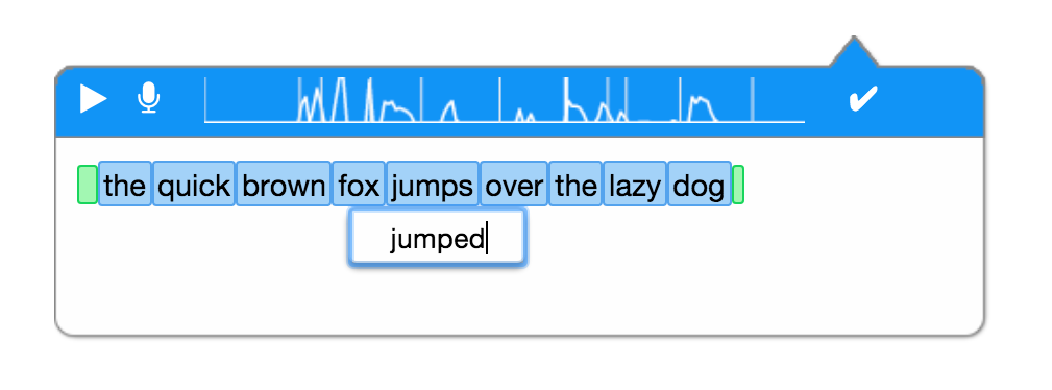
\includegraphics[width=\columnwidth,keepaspectratio]{figures/transcription_edit}
	\caption{To keep the user interface from becoming cluttered with secondary functionality, the transcription editing feature was implemented as a modal interaction. The pop-up box shown above ``opens'' the selected tokens for text editing in a separate control element, thus notifying the user that he or she is no longer directly editing the audio.}
	\label{fig:transcription}
\end{figure}


Our text-based approach to speech editing requires a reliable transcription as well as time intervals corresponding to each word.
Both of these requirements are fulfilled by the IBM Watson Developer Cloud speech-to-text transcription service, which is reported to have a word error rate of 10.4\% \cite{soltau:2014}.